\documentclass[aspectratio=169]{beamer} % O parâmetro aspectratio com valar 16:9 deixa o slide em widescreen

\usepackage[brazil]{babel}
\usepackage[utf8]{inputenc}
\usepackage[T1]{fontenc}

\usetheme{Madrid}
\setbeamertemplate{navigation symbols}{}

\title[Informática]{Informática}

\author[Diego S. C. Nascimento]{Diego Silveira Costa Nascimento}

\institute[IFRN]{
Instituto Federal de Educação, Ciência e Tecnologia do Rio Grande do Norte\\
diego.nascimento@ifrn.edu.br
}

\date[\today]{\today}

\begin{document}

\begin{frame}[plain]
	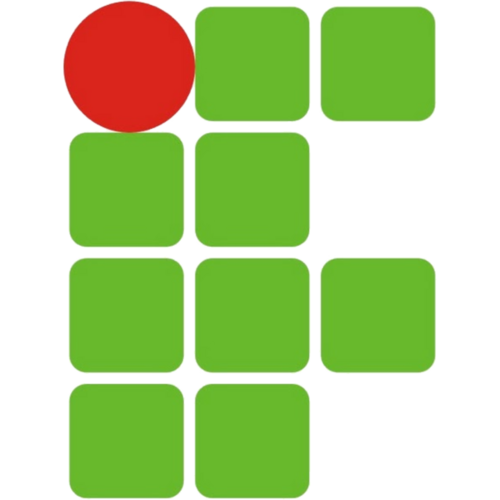
\includegraphics[scale=0.2]{img/IFRN}
	\titlepage
\end{frame}

\logo{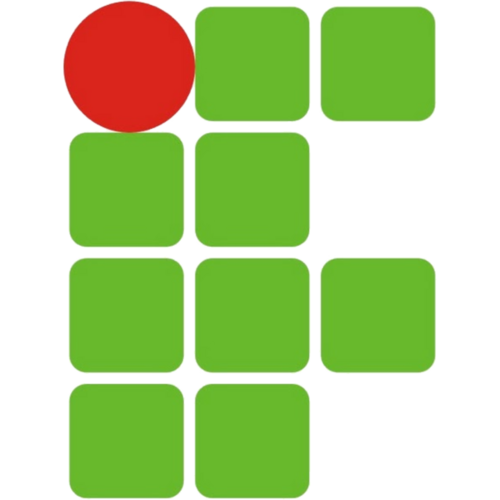
\includegraphics[scale=0.1]{img/IFRN}}

\begin{frame}
	\frametitle{Ementa do Curso}
  	\tableofcontents
\end{frame}

\AtBeginSection[]{
	\begin{frame}
		\frametitle{Ementa}
		\tableofcontents[currentsection]
	\end{frame}
}

\section{Introdução}

\begin{frame}
	\frametitle{História}
	
	\begin{itemize}
		\item Parte da evolução aconteceu ao mero acaso;
		\item A outra parte se deve a poucos homens que observaram os problemas cotidianos e tentaram encontrar um solução;
		\item Cada época apresentada seus principais pensadores, inventores e pessoas de diversos níveis de conhecimento;
		\item Para que uma invenção pudesse ser conhecida, havia uma demora de anos ou décadas; e
		\item O intervalo de conhecimento e de descobertas da humanidade vai diminuindo consideravelmente.
	\end{itemize}
\end{frame}

\begin{frame}
	\frametitle{As mãos}
	
	\begin{itemize}
		\item Primeira forma de mostrar uma quantidade; 
		\item Serviram como instrumentos de comparação; e
		\item Provavelmente aí está a origem do nosso sistema de numeração de base decimal (10 dedos).
	\end{itemize}\vfill
	
	\begin{exampleblock}{Ilustra\c cão}
		\begin{center}
			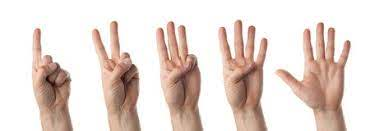
\includegraphics[scale=0.5]{img/dedos}
		\end{center}
	\end{exampleblock}
\end{frame}

\begin{frame}
	\frametitle{Objetos}
	
	\begin{itemize}
		\item Em latim, pedrinha se escreve \textit{calculu}.
	\end{itemize}\vfill
	
	\begin{exampleblock}{Ilustra\c cão}
		\begin{center}
			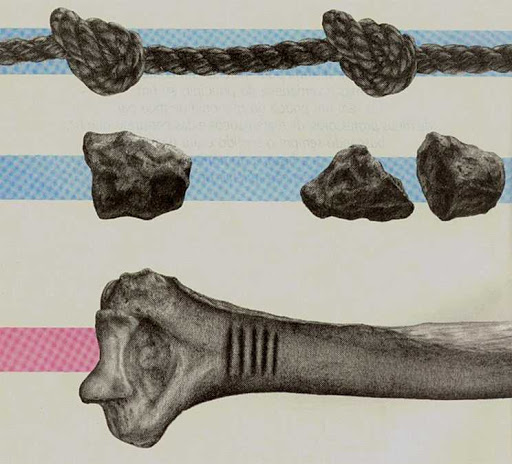
\includegraphics[scale=0.2]{img/objetos}
		\end{center}
	\end{exampleblock}
\end{frame}

\begin{frame}
	\frametitle{Ábaco}
	
	\begin{itemize}
		\item Provavelmente inventado na China (Dinastia de Yuan); e
		\item É o primeiro instrumento de calcular que se tem conhecimento.
	\end{itemize}\vfill
	
	\begin{exampleblock}{Ilustra\c cão}
		\begin{center}
			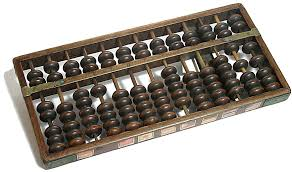
\includegraphics[scale=0.5]{img/abaco}
		\end{center}
	\end{exampleblock}
\end{frame}

\begin{frame}
	\frametitle{Ossos de Napier}
	
	\begin{itemize}
		\item John Napier foi um matemático escocês;
		\item Desenvolveu um conjunto de noves bastões chamados de Ossos de Napier; e
		\item Eram usados para multiplicar e dividir números elevados.
	\end{itemize}\vfill
	
	\begin{exampleblock}{Ilustra\c cão}
		\begin{center}
			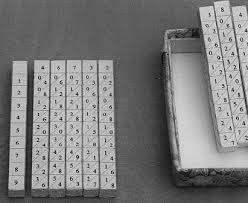
\includegraphics[scale=0.5]{img/ossos_napier}
		\end{center}
	\end{exampleblock}
\end{frame}

\begin{frame}
	\frametitle{Pascalina}
	
	\begin{itemize}
		\item Blaise Pascal, em 1642, inventou a primeira máquina de somar;
		\item Executava operações aritméticas quando se giravam os discos interligados; e
		\item Foi a precursora das calculadoras mecânicas.
	\end{itemize}\vfill
	
	\begin{exampleblock}{Ilustra\c cão}
		\begin{center}
			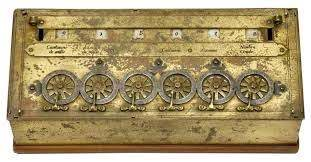
\includegraphics[scale=0.5]{img/pascalina}
		\end{center}
	\end{exampleblock}
\end{frame}

\begin{frame}
	\frametitle{Máquina de Leibniz}
	
	\begin{itemize}
		\item O alemão Gottfried Wilhelm Leibniz, em 1671, inventou uma máquina muito parecida com a Pascalina;
		\item Efetuava cálculos de multiplicação e divisão; e
		\item Se tornou a antecessora direta das calculadoras manuais.
	\end{itemize}\vfill
	
	\begin{exampleblock}{Ilustra\c cão}
		\begin{center}
			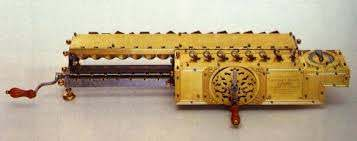
\includegraphics[scale=0.5]{img/maquina_leibniz}
		\end{center}
	\end{exampleblock}
\end{frame}

\begin{frame}
	\frametitle{Tear mecânico de Jacquard}
	
	\begin{itemize}
		\item Joseph-Marie Jacquard, em 1801, inventou um tear mecânico;
		\item Utilizava cartões perfurados;
		\item Fazia combinações de desenhos mais sofisticadas; e
		\item Cartões perfurados seriam posteriormente usados para projetar máquinas de calcular.
	\end{itemize}\vfill
	
	\begin{exampleblock}{Ilustra\c cão}
		\begin{center}
			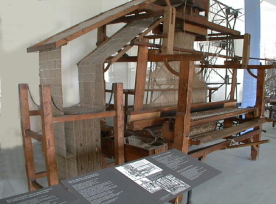
\includegraphics[scale=0.5]{img/tear_jacquard}
		\end{center}
	\end{exampleblock}
\end{frame}

\begin{frame}
	\frametitle{Máquina diferencial}
	
	\begin{itemize}
		\item Charles Babbage é conhecido como o \structure{Pai da Computação};
		\item Em 1822, desenvolveu a máquina diferencial de Babbage; 
		\item Permitia cálculos de funções trigonométricas e logarítmicas; e 
		\item Utilizava os cartões de Jacquard.
	\end{itemize}\vfill
	
	\begin{exampleblock}{Ilustra\c cão}
		\begin{center}
			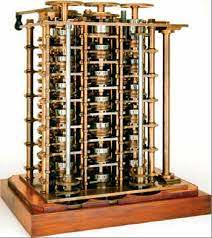
\includegraphics[scale=0.5]{img/maquina_diferencial}
		\end{center}
	\end{exampleblock}
\end{frame}

\begin{frame}
	\frametitle{Máquina analítica}
	
	\begin{itemize}
		\item Charles Babbage, em 1834, desenvolveu a máquina analítica;
		\item Permitia somar, dividir, subtrair e multiplicar;
		\item Armazenava dados em memória de até 1000 números de 50 dígitos; e 
		\item Imprimia resultados;
	\end{itemize}\vfill
	
	\begin{exampleblock}{Ilustra\c cão}
		\begin{center}
			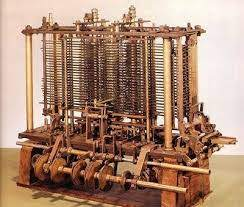
\includegraphics[scale=0.5]{img/maquina_analitica}
		\end{center}
	\end{exampleblock}
\end{frame}

\begin{frame}
	\frametitle{Tabulador de Hollerith}
	
	\begin{itemize}
		\item Desenvolvida para o censo dos EUA;
		\item  Hermann Hollerith percebeu que só terminaria de apurar os dados do censo quando já seria o tempo de se efetuar novo censo;
		\item Integrou a ideia dos cartões de Jacquard e do conceito de impulsos elétricos para a transmissão de dados;
		\item Tabulating Machine Company (1896); e
		\item Em 1924, tornou-se a International Business Machines Corporation – IBM.
	\end{itemize}\vfill
	
	\begin{exampleblock}{Ilustra\c cão}
		\begin{center}
			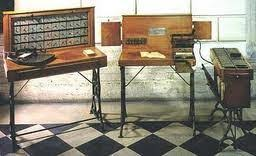
\includegraphics[scale=0.5]{img/tabulador_hollerith}
		\end{center}
	\end{exampleblock}
\end{frame}

\begin{frame}
	\frametitle{Computômetro}
	
	\begin{itemize}
		\item Foi desenvolvido por  Dorr Eugene Felt em 1887; e
		\item Primeira máquina com teclado para somar e imprimir.
	\end{itemize}\vfill
	
	\begin{exampleblock}{Ilustra\c cão}
		\begin{center}
			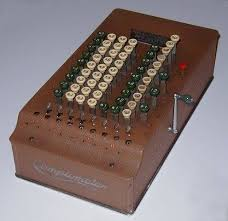
\includegraphics[scale=0.5]{img/computometro}
		\end{center}
	\end{exampleblock}
\end{frame}

\begin{frame}
	\frametitle{Mark I}
	
	\begin{itemize}
		\item Foi desenvolvido por Howard Aiken em 1937;
		\item Foi o primeiro computador eletromecânico, construído na Universidade de Harvard;
		\item Ajuda financeira da IBM: US\$ 500.000,00;
		\item Controlado por programa e usava o sistema decimal;
		\item Cerca de 15m de comprimento e 2,5m de altura; e
		\item Realizava uma soma em 0,3s, uma multiplicação em 0,4s e uma divisão em cerca de 10s.
	\end{itemize}\vfill
	
	\begin{exampleblock}{Ilustra\c cão}
		\begin{center}
			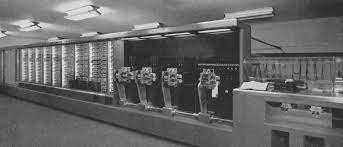
\includegraphics[scale=0.5]{img/marki}
		\end{center}
	\end{exampleblock}
\end{frame}

\begin{frame}
	\frametitle{Série Z1, Z2, Z3, Z4 e Z5}
	
	\begin{itemize}
		\item Desenvolvido pelo engenheiro alemão Konrad Zuse;
		\item  Computador construído à base de relés; e
		\item Os cálculos eram baseados em aritmética binária.
	\end{itemize}\vfill
	
	\begin{exampleblock}{Ilustra\c cão}
		\begin{center}
			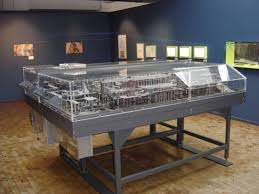
\includegraphics[scale=0.5]{img/z1}
		\end{center}
	\end{exampleblock}
\end{frame}

\begin{frame}
	\frametitle{Colossus}
	
	\begin{itemize}
		\item Projetado pelo matemático britânico Alan Turing em 1944;
		\item Usado para decifrar os códigos de Hitler na Segunda Gerra Mundial; e
		\item Ao invés de relés eletromecânicos, usava 2.000 válvulas eletrônicas.
	\end{itemize}\vfill
	
	\begin{exampleblock}{Ilustra\c cão}
		\begin{center}
			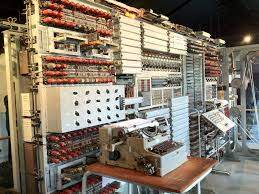
\includegraphics[scale=0.5]{img/colossus}
		\end{center}
	\end{exampleblock}
\end{frame}

\begin{frame}
	\frametitle{ENIAC}
	
	\begin{itemize}
		\item John Eckert e John Mauchly construíram o Eletronic Numerical Integrator and Calculator (ENIAC) em 1946;
		\item Primeiro computador eletrônico digital de propósito geral;
		\item Consumo cerca de 200 KW de potência;
		\item Memória podia registrar até 20 números de 10 dígitos cada um; e 
		\item Fazia 5.000 adições e 360 multiplicações por segundo.
	\end{itemize}\vfill
	
	\begin{exampleblock}{Ilustra\c cão}
		\begin{center}
			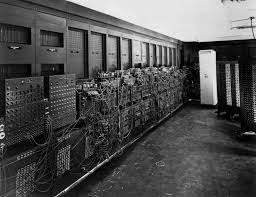
\includegraphics[scale=0.4]{img/eniac}
		\end{center}
	\end{exampleblock}
\end{frame}

\begin{frame}
	\frametitle{UNIVAC}
	
	\begin{itemize}
		\item John Eckert e John Mauchly construíram o Universal Automatic Computer (UNIVAC) em 1951;
		\item Primeiro computador comercial entregue a um cliente; e
		\item Era um ENIAC modificado.
	\end{itemize}\vfill
	
	\begin{exampleblock}{Ilustra\c cão}
		\begin{center}
			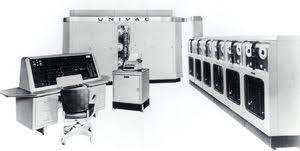
\includegraphics[scale=0.5]{img/univac}
		\end{center}
	\end{exampleblock}
\end{frame}

\begin{frame}
	\frametitle{TRADIC}
	
	\begin{itemize}
		\item Jean Howard Felker  construiu o Transistor Digital Computer (TRADIC) em 1954; e
		\item Primeiro computador 100\% transistorizado.
	\end{itemize}\vfill
	
	\begin{exampleblock}{Ilustra\c cão}
		\begin{center}
			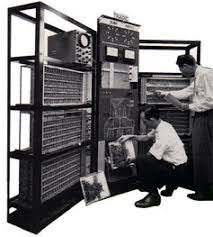
\includegraphics[scale=0.5]{img/tradic}
		\end{center}
	\end{exampleblock}
\end{frame}

\begin{frame}
	\frametitle{IBM 1401}
	
	\begin{itemize}
		\item Desenvolvido em 1959; 
		\item Totalmente transistorizado;
		\item Possuía capacidade de memória base de 4.096 bytes operando em ciclos de memória de 12 microssegundos; e
		\item Utilizado em vários seguimentos de mercados, principalmente por bancos.
	\end{itemize}\vfill
	
	\begin{exampleblock}{Ilustra\c cão}
		\begin{center}
			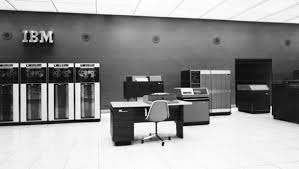
\includegraphics[scale=0.5]{img/ibm1401}
		\end{center}
	\end{exampleblock}
\end{frame}

\begin{frame}
	\frametitle{IBM System 360}
	
	\begin{itemize}
		\item Lançado em 1964; 
		\item Utilizava circuitos integrados; e 
		\item Constituia uma família de mainframes.
	\end{itemize}\vfill
	
	\begin{exampleblock}{Ilustra\c cão}
		\begin{center}
			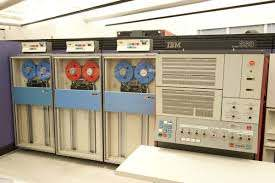
\includegraphics[scale=0.5]{img/ibm360}
		\end{center}
	\end{exampleblock}
\end{frame}

\begin{frame}
	\frametitle{Apple I}
	
	\begin{itemize}
		\item Steve Jobs e Steve Wozniak construíram o Apple I em 1976;
		\item Era uma placa de circuito impresso totalmente montada, contendo cerca de 30 chips;
		\item Um microprocessador MOS 6502 de 1 MHz;
		\item 4 k de memória;
		\item Tinham de acrescentar um gabinete, fonte de energia, teclado e monitor; e
		\item Permitia placa de expansão, contendo uma interface para cassetes, utilizados no armazenamento dos dados e programas.
	\end{itemize}\vfill
	
	\begin{exampleblock}{Ilustra\c cão}
		\begin{center}
			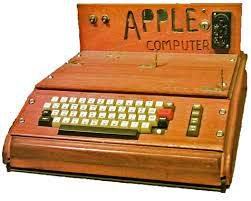
\includegraphics[scale=0.4]{img/apple1}
		\end{center}	
	\end{exampleblock}
\end{frame}

\begin{frame}
	\frametitle{Apple II}
	
	\begin{itemize}
		\item Lançado em 1977;
		\item Foi um sucesso no mercado de microcomputadores; 
		\item Possuia monitor e teclado juntos; e
		\item Memória RAM de 16 KB.
	\end{itemize}\vfill
	
	\begin{exampleblock}{Ilustra\c cão}
		\begin{center}
			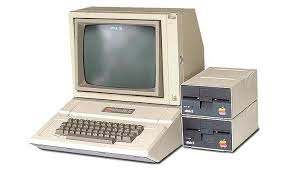
\includegraphics[scale=0.4]{img/apple2}
		\end{center}	
	\end{exampleblock}
\end{frame}

\begin{frame}
	\frametitle{IBM PC}
	
	\begin{itemize}
		\item Anunciado em 1981;
		\item Usava processador Intel 8086 de 4.77 MHz; e
		\item Possuia disquete com capacidade de armazenamento de 160 KB.
	\end{itemize}\vfill
	
	\begin{exampleblock}{Ilustra\c cão}
		\begin{center}
			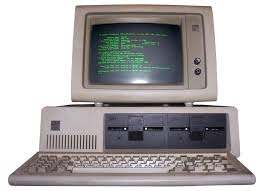
\includegraphics[scale=0.4]{img/ibmpc}
		\end{center}		
	\end{exampleblock}
\end{frame}

\begin{frame}
	\frametitle{Compaq Portable}
	
	\begin{itemize}
		\item Lançado em 1982
		\item Usava processador Intel 80286; 
		\item Possuia memória RAM de 16 MB; e 
		\item Pesava em torno de 11 kg.
	\end{itemize}\vfill
	
	\begin{exampleblock}{Ilustra\c cão}
		\begin{center}
			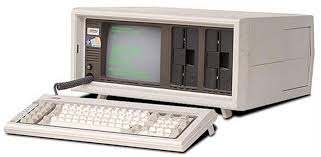
\includegraphics[scale=0.4]{img/compac_portable}
		\end{center}			
	\end{exampleblock}
\end{frame}

\begin{frame}
	\frametitle{Lisa}
	
	\begin{itemize}
		\item Lança em 1982 pela Apple;
		\item Trazia um mouse;
		\item Possuia interface gráfica;
		\item Disquetes com capacidade de armazenamento de 260 KB; e 
		\item Trazia um disco rígido (winchester) com capacidade de 10 MB de armazenamento.
	\end{itemize}\vfill
	
	\begin{exampleblock}{Ilustra\c cão}
		\begin{center}
			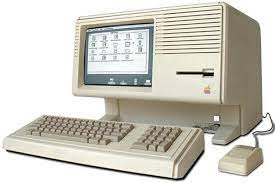
\includegraphics[scale=0.4]{img/lisa}
		\end{center}			
	\end{exampleblock}
\end{frame}

\begin{frame}
	\frametitle{Macintosh}
	
	\begin{itemize}
		\item Lança em 1984 pela Apple;
		\item  Nome inspirado em uma espécie de maçã canadense; e
		\item Possuia interface gráfica mais amigável.
	\end{itemize}\vfill
	
	\begin{exampleblock}{Ilustra\c cão}
		\begin{center}
			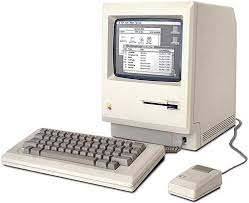
\includegraphics[scale=0.4]{img/macintosh}
		\end{center}			
	\end{exampleblock}
\end{frame}

\begin{frame}
	\frametitle{Tecnologias Disponívies}
	
	\begin{itemize}
		\item Desktop;
		\item Notebook;
		\item Smartphone;
		\item Tablet;
		\item Smartwatch; e
		\item Smartglass.
	\end{itemize}
\end{frame}

\begin{frame}
	\frametitle{Ergonomia no Uso dos Computadores}

\begin{columns}

\column{0.6\textwidth}
	\begin{itemize}
		\item Visa buscar os efeitos desejados, simultaneamente, de: o Conforto, a Segurança e por fim a Eficiência (RN--17 do Ministério do Trabalho e Previdência Social);
		\item  Reduzir os riscos em contrair doenças músculo-esqueléticas como a LER/DORT, dores e lesões da coluna.
		\item Para o uso correto do computador, é preciso se ater aos detalhes para:
		\begin{itemize}
			\item Visão;
			\item Punhos e bra\c cos;
			\item Costas; e
			\item Pés.
		\end{itemize}
	\end{itemize}

\column{0.3\textwidth}
	\begin{exampleblock}{Ilustra\c cão}
		\begin{center}
			
\includegraphics[scale=0.4]{img/ergonomia}
		\end{center}			
	\end{exampleblock}

\end{columns}	
\end{frame}

\begin{frame}
	\frametitle{Ergonomia da Visão}
	
	\begin{itemize}
		\item Para conseguir um conforto visual é preciso que o monitor esteja distante dos seus olhos entre 45cm e 70cm. 
		\item A altura também é muito importante, tenha o topo do monitor alinhado horizontalmente com seus olhos. 
		\item Observe para não inclinar a cabeça para baixo.
	\end{itemize}
\end{frame}

\begin{frame}
	\frametitle{Ergonomia dos Punhos e Braços}
	
	\begin{itemize}
		\item Os cotovelos devem manter um ângulo de 90$^{\circ}$;
		\item Os braços e os punhos devem ter os ângulos certos e o uso de apoios é fundamental. 
		\item O teclado deve ser regulável e deve estar alinhado aos cotovelos.
	\end{itemize}
\end{frame}

\begin{frame}
	\frametitle{Ergonomia das Costas}
	
	\begin{itemize}
		\item Nas costas é fundamental que a coluna esteja em 90$^{\circ}$ com as pernas. 
		\item Na região lombar deve-se usar um apoio, muitas vezes ajustado pela própria cadeira. 
		\item O encosto de tamanho médio ao seu corpo ajuda muito a garantir conforto.
	\end{itemize}
\end{frame}

\begin{frame}
	\frametitle{Ergonomia dos Pés}
	
	\begin{itemize}
		\item Os pés precisam estar no chão, não podem ficar suspensos. 
		\item Muitas vezes pela regulagem da mesa isso não ocorre, e o uso de apoios para os pés se faz necessário. 
		\item Observe bem esse aspecto, evite dores e desconforto.
	\end{itemize}
\end{frame}

\section{Hardware}

\begin{frame}
	\frametitle{Hardware}
	
	\begin{block}{Defini\c cão}
		É toda parte física de um computador, ou seja, é o conjunto de componentes eletrônicos, circuitos integrados e placas, que se comunicam através de barramento.
	\end{block}
\end{frame}

\begin{frame}
	\frametitle{Placa-mãe}
	
	\begin{block}{Defini\c cão}
		É a parte responsável por conectar e interligar todos os componentes (periféricos) do computador: processador, memória, disco rígido, placa gráfica, entre outros.
	\end{block}\vfill
	
	\begin{exampleblock}{Ilustra\c cão}
		\begin{center}
			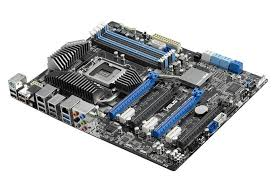
\includegraphics[scale=0.4]{img/placa-mae}
		\end{center}			
	\end{exampleblock}
\end{frame}

\begin{frame}
	\frametitle{Processador}
	
	\begin{block}{Defini\c cão}
		É a unidade central de computador (CPU) responsável por realizar as funções de cálculo e tomada de decisão de um computador.
	\end{block}\vfill
	
	\begin{itemize}
		\item Unidade lógica e aritmética (ULA);
		\item Unidade de controle (UC); e
		\item Registradores.
	\end{itemize}\vfill
	
	\begin{exampleblock}{Ilustra\c cão}
		\begin{center}
			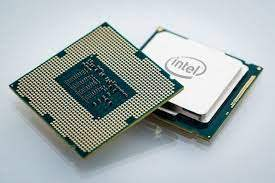
\includegraphics[scale=0.4]{img/processador}
		\end{center}
	\end{exampleblock}
\end{frame}

\begin{frame}
	\frametitle{Memória}
	
	\begin{block}{Defini\c cão}
		São todos os dispositivos que permitem ao computador guardar dados, temporariamente ou permanentemente.
	\end{block}\vfill
	
	\begin{itemize}
		\item ROM;
		\item RAM; e 
		\item Cache.
	\end{itemize}
\end{frame}

\begin{frame}
	\frametitle{Memória ROM}
		
	\begin{itemize}
		\item Um acrônimo para \underline{R}ead \underline{O}nly \underline{M}emory;
		\item Nela estão gravadas as características do computador; e
		\item Vem de fábrica com toda rotina necessária e não pode ser alterada.
	\end{itemize}\vfill
	
	\begin{exampleblock}{Ilustra\c cão}
		\begin{center}
			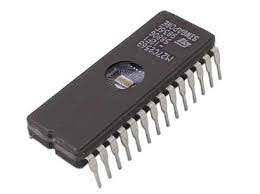
\includegraphics[scale=0.4]{img/rom}
		\end{center}		
	\end{exampleblock}
\end{frame}

\begin{frame}
	\frametitle{Memória RAM}
		
	\begin{itemize}
		\item Um acrônimo para \underline{R}andom \underline{A}ccess \underline{M}emory; 
		\item É completamente volátil; e
		\item Os dados só permanecem armazenados enquanto houver corrente elétrica.
	\end{itemize}\vfill
	
	\begin{exampleblock}{Ilustra\c cão}
		\begin{center}
			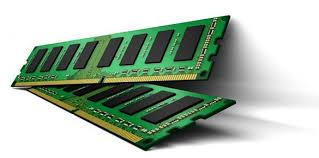
\includegraphics[scale=0.4]{img/ram}
		\end{center}		
	\end{exampleblock}
\end{frame}

\begin{frame}
	\frametitle{Memória Cache}
		
	\begin{itemize}
		\item É um dispositivo de acesso rápido; e
		\item Tem a finalidade de acelerar a velocidade da memória RAM.
	\end{itemize}\vfill
	
	\begin{exampleblock}{Ilustra\c cão}
		\begin{center}
			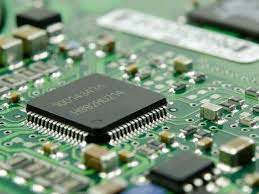
\includegraphics[scale=0.4]{img/cache}
		\end{center}		
	\end{exampleblock}
\end{frame}

\begin{frame}
	\frametitle{Tipos de Periféricos}
		
	\begin{itemize}
		\item Entrada;
		\item Saída; e
		\item Entrada e Saída.
	\end{itemize}
\end{frame}

\begin{frame}
	\frametitle{Periféricos de entrada}
	
	\begin{block}{Defini\c cão}
		São todos os elementos que têm por finalidade realizar a entrada de dados no computador.
	\end{block}\vfill
	
	\begin{itemize}
		\item Teclado;
		\item Mouse;
		\item Scanner;
		\item Webcam;
		\item Microfone;
		\item Leitor de código de barras;
		\item Leitores biométricos; e
		\item Mesa digitalizadora.
	\end{itemize}
\end{frame}

\begin{frame}
	\frametitle{Teclado}
	
	\begin{block}{Defini\c cão}
		O teclado de computador é um tipo de periférico de entrada utilizado pelo usuário para a entrada manual no sistema de dados e comandos.
	\end{block}\vfill
	
	\begin{exampleblock}{Ilustra\c cão}
		\begin{center}
			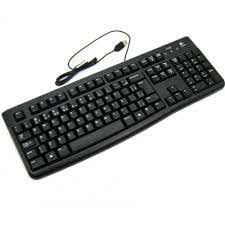
\includegraphics[scale=0.4]{img/teclado}
		\end{center}
	\end{exampleblock}
\end{frame}

\begin{frame}
	\frametitle{Mouse}
	
	\begin{block}{Defini\c cão}
		É um periférico de entrada que, historicamente, se juntou ao teclado como auxiliar no processo de entrada de dados, especialmente em programas com interface gráfica.
	\end{block}\vfill
	
	\begin{exampleblock}{Ilustra\c cão}
		\begin{center}
			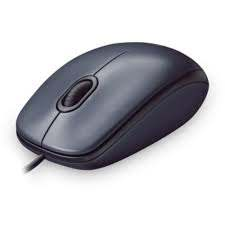
\includegraphics[scale=0.4]{img/mouse}
		\end{center}		
	\end{exampleblock}
\end{frame}

\begin{frame}
	\frametitle{Scanner}
	
	\begin{block}{Defini\c cão}
		É um periférico de entrada responsável por digitalizar imagens, fotos e textos impressos para o computador de forma estática.
	\end{block}\vfill
	
	\begin{exampleblock}{Ilustra\c cão}
		\begin{center}
			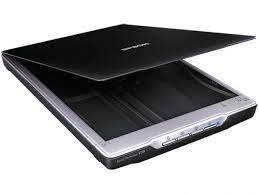
\includegraphics[scale=0.4]{img/scanner}
		\end{center}				
	\end{exampleblock}
\end{frame}

\begin{frame}
	\frametitle{Webcam}
	
	\begin{block}{Defini\c cão}
		É um periférico de entrada responsável por digitalizar vídeos para o computador.
	\end{block}\vfill
	
	\begin{exampleblock}{Ilustra\c cão}
		\begin{center}
			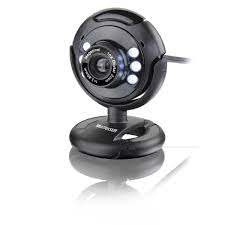
\includegraphics[scale=0.4]{img/webcam}
		\end{center}				
	\end{exampleblock}
\end{frame}

\begin{frame}
	\frametitle{Microfone}
	
	\begin{block}{Defini\c cão}
		É um periférico de entrada responsável capturar som para o computador.
	\end{block}\vfill
	
	\begin{exampleblock}{Ilustra\c cão}
		\begin{center}
			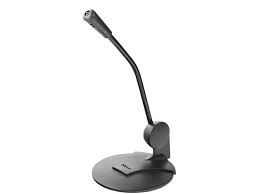
\includegraphics[scale=0.4]{img/microfone}
		\end{center}				
	\end{exampleblock}
\end{frame}

\begin{frame}
	\frametitle{Leitor de Código de Barras}
	
	\begin{block}{Defini\c cão}
		É um periférico de entrada que permite a leitura de códigos que são representados no formato em barras.
	\end{block}\vfill
	
	\begin{exampleblock}{Ilustra\c cão}
		\begin{center}
			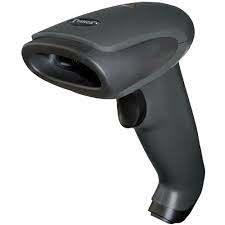
\includegraphics[scale=0.4]{img/leitor_de_codigo_de_barras}
		\end{center}				
	\end{exampleblock}
\end{frame}

\begin{frame}
	\frametitle{Leitor de Biométrico}
	
	\begin{block}{Defini\c cão}
		É um dispositivo de entrada que permite a leitura de características físicas ou comportamentais dos seres vivos.
	\end{block}\vfill
	
	\begin{exampleblock}{Ilustra\c cão}
		\begin{center}
			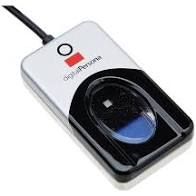
\includegraphics[scale=0.5]{img/leitor_biometrico}
		\end{center}		
	\end{exampleblock}
\end{frame}

\begin{frame}
	\frametitle{Mesa Digitalizadora}
	
	\begin{block}{Defini\c cão}
		É um dispositivo de entrada que permite a leitura de gráficos realizados a parte de uma caneta específica.
	\end{block}\vfill
	
	\begin{exampleblock}{Ilustra\c cão}
		\begin{center}
			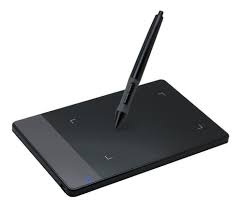
\includegraphics[scale=0.5]{img/mesa_digitalizadora}
		\end{center}		
	\end{exampleblock}
\end{frame}


\begin{frame}
	\frametitle{Periféricos de Saída}
	
	\begin{block}{Defini\c cão}
		E todo e qualquer elemento que compõe o computador cuja finalidade é a saída dos dados.
	\end{block}\vfill
	
	\begin{itemize}
		\item Monitor; e
		\item Impressora.
	\end{itemize}
\end{frame}

\begin{frame}
	\frametitle{Monitor}
	
	\begin{block}{Defini\c cão}
		O monitor é um dispositivo de saída do computador, cuja função é transmitir informação ao utilizador através da imagem.
	\end{block}\vfill
	
	\begin{exampleblock}{Ilustra\c cão}
		\begin{center}
			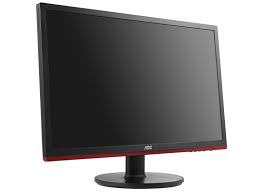
\includegraphics[scale=0.4]{img/monitor}
		\end{center}		
	\end{exampleblock}
\end{frame}

\begin{frame}
	\frametitle{Impressora}
	
	\begin{block}{Defini\c cão}
		É um periférico de saída que permite reproduzir textos, gráficos ou qualquer outro resultado de uma aplicação.
	\end{block}\vfill
	
	\begin{exampleblock}{Ilustra\c cão}
		\begin{center}
			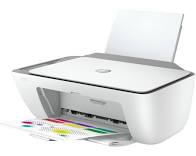
\includegraphics[scale=0.5]{img/impressora}
		\end{center}		
	\end{exampleblock}
\end{frame}

\begin{frame}
	\frametitle{Periféricos de Entrada e Saída}
	
	\begin{block}{Defini\c cão}
		É todo e qualquer elemento que compõe o computador cuja finalidade é entrada e saída dos dados.
	\end{block}\vfill
	
	\begin{itemize}
		\item Fita DAT;
		\item Disco rígido;
		\item Disquete;
		\item CD, DVD e Disco Blu-ray; 
		\item Pendrive; e
		\item Cartão.
	\end{itemize}
\end{frame}

\begin{frame}
	\frametitle{Fita DAT}
		
	\begin{itemize}
		\item É uma mídia de armazenamento não-volátil;
		\item Consiste em uma fita plástica coberta de material magnetizável; e 
		\item Pode ser utilizada para registro de informações analógicas ou digitais.
	\end{itemize}\vfill
	
	\begin{exampleblock}{Ilustra\c cão}
		\begin{center}
			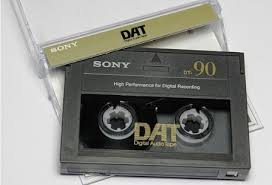
\includegraphics[scale=0.4]{img/fita_dat}
		\end{center}		
	\end{exampleblock}
\end{frame}

\begin{frame}
	\frametitle{Disco Rígido}
		
	\begin{itemize}
		\item Conhecidos como Hard Disk (HD) ou winchester;
		\item É uma memória não-volátil; e
		\item É a parte do computador onde são armazenados os dados.
	\end{itemize}\vfill
	
	\begin{exampleblock}{Ilustra\c cão}
		\begin{center}
			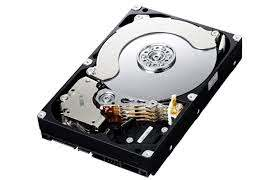
\includegraphics[scale=0.4]{img/hd}
		\end{center}		
	\end{exampleblock}
\end{frame}

\begin{frame}
	\frametitle{Disquete}
		
	\begin{itemize}
		\item Também conhecido como floppy disk; e
		\item É um disco de armazenamento magnético;
		\item Fino e flexível, selado por um plástico retangular; e 
		\item Forrado com tecido que remove as partículas de poeira.
	\end{itemize}\vfill
	
	\begin{exampleblock}{Ilustra\c cão}
		\begin{center}
			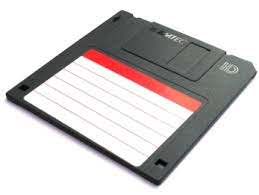
\includegraphics[scale=0.4]{img/disquete}
		\end{center}
	\end{exampleblock}
\end{frame}

\begin{frame}
	\frametitle{CD, DVD e Disco Blu-ray}
		
	\begin{itemize}
		\item São dispositivos de armazenamento por meio óptico; e
		\item A leitura e escrita das informações se dá por meio de um feixe laser de alta precisão.
	\end{itemize}\vfill
	
	\begin{exampleblock}{Ilustra\c cão}
		\begin{center}
			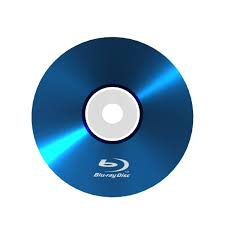
\includegraphics[scale=0.4]{img/cd}
		\end{center}
	\end{exampleblock}
\end{frame}

\begin{frame}
	\frametitle{Pendrive}
		
	\begin{itemize}
		\item É um dispositivo de memória constituído por memória flash; e 
		\item Utiliza porta USB.
	\end{itemize}\vfill
	
	\begin{exampleblock}{Ilustra\c cão}
		\begin{center}
			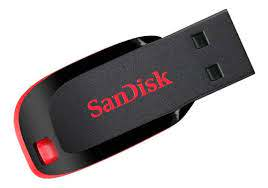
\includegraphics[scale=0.4]{img/pendrive}
		\end{center}
	\end{exampleblock}
\end{frame}

\begin{frame}
	\frametitle{Cartão de Memória}
		
	\begin{itemize}
		\item É um dispositivo de memória constituído por memória flash; e 
		\item Ideal para equipamentos móveis.
	\end{itemize}\vfill
	
	\begin{exampleblock}{Ilustra\c cão}
		\begin{center}
			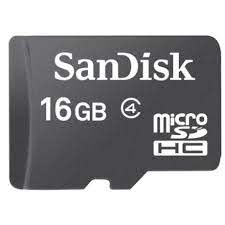
\includegraphics[scale=0.4]{img/cartao_de_memoria}
		\end{center}
	\end{exampleblock}
\end{frame}

\section{Software}

\begin{frame}
	\frametitle{Software}
		
	\begin{block}{Defini\c cão}
		É uma sequência de instruções escritas para serem interpretadas por um computador com o objetivo de executar tarefas específicas.
	\end{block}\vfill
	
	Tipos:
	\begin{itemize}
		\item Softwares de sistema; e
		\item Softwares aplicativos.
	\end{itemize}
\end{frame}

\begin{frame}
	\frametitle{Software de Sistema}
		
	\begin{itemize}
		\item Abrange todos os programas relacionados com a coordenação operacional do computador, dentre eles o sistema operacional; e
		\item Coordena a interação entre hardware e software, principalmente a transferência de informações entre a memória e os dispositivos de entrada e saída.
	\end{itemize}\vfill
	
	\begin{exampleblock}{Ilustra\c cão}
		\begin{columns}[c]
			\column{.3\textwidth}
				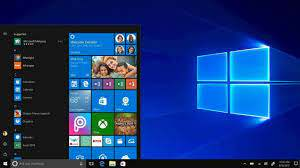
\includegraphics[scale=0.4]{img/windows}
		
			\column{.3\textwidth}
				\includegraphics[scale=0.4]{img/macos}
			
			\column{.3\textwidth}
				\includegraphics[scale=0.4]{img/ubuntu}
		\end{columns}
	\end{exampleblock}
\end{frame}

\begin{frame}
	\frametitle{Software Aplicativo}
		
	\begin{itemize}
		\item Conjunto de programas desenvolvidos para realizar tarefas ou processos específicos, em geral, relacionados com a geração de informação;
		\item Opera juntamente com o sistema operacional para que um usuário execute tarefas com o computador sem necessitar ser um desenvolvedor de software;	
		\item Podem ser personalizados ou oferecidos em pacotes; e
		\item Software comercial é vendido em lojas ou por meio de catálogos.
	\end{itemize}
\end{frame}

\begin{frame}
	\frametitle{Tipos de Software Aplicativo}
		
	\begin{itemize}
		\item Escritório; 
		\item Administrativos; 
		\item Automação Comercial; 
		\item Técnico-científicos; 
		\item Automação Industrial; 
		\item Apoio Educacional;  e 
		\item Entretenimento.
	\end{itemize}
\end{frame}

\begin{frame}
	\frametitle{Editor de Texto}
		
	\begin{itemize}
		\item Software de computador mais amplamente usado;
		\item Permite criar, editar, formatar e imprimir em um documento; e 
		\item Exemplos: Microsoft Word, LibreOffice Writer, Apple Pages e Google Documentos.
	\end{itemize}\vfill
	
	\begin{exampleblock}{Ilustra\c cão}
		\begin{center}
			\includegraphics[scale=0.4]{img/word}
		\end{center}	
	\end{exampleblock}
\end{frame}

\begin{frame}
	\frametitle{Planilhas Eletrônicas}
		
	\begin{itemize}
		\item Compostas de colunas e linhas;
		\item Usadas como uma ferramenta de negócio;
		\item Recalcula de maneira automática os resultados quando um número é alterado; e
		\item Exemplos: Microsoft Excel, LibreOffice Calc, Apple Numbers e Google Planilhas.
	\end{itemize}\vfill
	
	\begin{exampleblock}{Ilustra\c cão}
		\begin{center}
			\includegraphics[scale=0.4]{img/excel}
		\end{center}		
	\end{exampleblock}
\end{frame}

\begin{frame}
	\frametitle{Editores de Apresenta\c cão}
		
	\begin{itemize}
		\item O software de apresentação gráfica pode produzir gráficos, mapas e tabelas, detectar tendências mais facilmente e tomar decisões mais rapidamente, já que a informação visual é mais atraente do que uma página numérica;
		\item Exemplos: Microsoft Power Point, LibreOffice Impress, Apple Keynote e Google Apresenta\c cões.
	\end{itemize}\vfill
	
	\begin{exampleblock}{Ilustra\c cão}
		\begin{center}
			\includegraphics[scale=0.4]{img/powerpoint}
		\end{center}
	\end{exampleblock}
\end{frame}

\begin{frame}
	\frametitle{Produ\c cão Gráfica}
		
	\begin{itemize}
		\item O software gráfico permite a manipulação de imagens; e
		\item  Exemplos: Inkscape, Gimp, Photoshop, Corel Draw, Afinity Designer e iMove.
	\end{itemize}\vfill
	
	\begin{exampleblock}{Ilustra\c cão}
		\begin{center}
			\includegraphics[scale=0.4]{img/afinity}
		\end{center}
	\end{exampleblock}
\end{frame}

\begin{frame}
	\frametitle{Gerenciamento de Informações Pessoais}
		
	\begin{itemize}
		\item Oferecem funções para controlar as atividades de uma vida atarefada;
		\item Recursos de calendário, catálogo de endereços, gerenciador de tarefas, bloco de notas e calculadora; e
		\item Exemplos:  Microsoft Outlook, Microsoft OneNote, Google Agenda e Evernote.
	\end{itemize}\vfill
	
	\begin{exampleblock}{Ilustra\c cão}
		\begin{center}
			\includegraphics[scale=0.4]{img/agenda}
		\end{center}	
	\end{exampleblock}
\end{frame}

\begin{frame}
	\frametitle{Comunica\c cão}
		
	\begin{itemize}
		\item O software de comunicação permite que dois ou mais dispositivos se comuniquem reciprocamente; e
		\item Atualmente a internet é o meio mais provável de comunicação tanto de indivíduos quanto de empresas.
		\item Exemplos: Skype, Google Meet, Microsoft Teams, Google Chrome e E-mail.
	\end{itemize}\vfill
	
	\begin{exampleblock}{Ilustra\c cão}
		\begin{center}
			\includegraphics[scale=0.4]{img/teams}
		\end{center}
	\end{exampleblock}
\end{frame}

\begin{frame}
	\frametitle{Licen\c cas de Software}

	\begin{block}{Defini\c cão}
		É um direito de propriedade intelectual que define os termos de utiliza\c cão ou distribui\c cão dos softwares.
	\end{block}\vfill
		
	Tipos de Licen\c ca:
	\begin{itemize}
		\item Freeware;
		\item Shareware;
		\item Licen\c ca de Aquisi\c cão Perpétua;
		\item Software Proprietário;
		\item Software as a service (SAAS);
		\item Software Livre;
		\item Open Source;
		\item AdWare; e
		\item End User License Agreement (EULA).
	\end{itemize}
\end{frame}

\begin{frame}
	\frametitle{Vírus de Computador}

	\begin{block}{Defini\c cão}
		É um software que foi desenvolvido para se replicar de forma autônoma com fins maliciosos.
	\end{block}\vfill
		
	Tipos de vírus:
	\begin{itemize}
		\item Vírus de Boot;
		\item Time Bomb;
		\item Worm;
		\item Trojans;
		\item Hijackers;
		\item Estado Zombie;
		\item Vírus de Macro; e
		\item Spyware.
	\end{itemize}
\end{frame}

\section{Sistema Operacional}

\begin{frame}
	\frametitle{Sistema Operacional}
	
	\begin{block}{Defini\c cão}
		Um conjunto de programas cuja função é gerenciar os recursos do sistema fornecendo uma interface entre o computador e o usuário.
	\end{block}
\end{frame}

\begin{frame}
	\frametitle{Características de um Sistema Operacional}
		
	\begin{itemize}
		\item \structure{Multitarefa}  – Capacidade de executar dois ou mais programas, no mesmo intervalo de tempo, de maneira concorrente, controlados por eventos;
		\item \structure{Multiprocessamento} – Capacidade de usar e gerenciar mais de um processador simultaneamente; e
		\item \structure{Multiusuário} – Permite que mais de um usuário acesse o computador ao mesmo tempo.
	\end{itemize}
\end{frame}

\begin{frame}
	\frametitle{Funções do Sistema Operacional}
		
	\begin{itemize}
		\item Gerenciamento da memória;
		\item Gestão do sistema de armazenamento e de arquivos; 
		\item Gestão e configuração de dispositivos;
		\item Gestão e suporte a outros programas; 
		\item Interface com o usuário;
		\item Programação de tarefas;
		\item Segurança do sistema;
		\item Controle da rede; e
		\item Monitoração do desempenho.
	\end{itemize}
\end{frame}

\begin{frame}
	\frametitle{Sistemas Operacionais mais Conhecidos}
		
	\begin{itemize}
		\item Windows;
		\item Mac OS;
		\item Linux;
		\item Chrome OS; e
		\item Free BSD.
	\end{itemize}
\end{frame}

\section{Internet}

\begin{frame}
	\frametitle{Internet}
		
	\begin{block}{Defini\c cão}
		É o maior conglomerado de redes de comunicações em escala mundial.
	\end{block} \vfill
	
	\begin{itemize}
		\item É formada por vários computadores e dispositivos conectados em uma rede mundial;
		\item Dispõe milhões de dispositivos interligados por um protocolo de comunicação; e
		\item Permite o acesso a informações e todo tipo de transferência de dados.
	\end{itemize}\vfill
	
	\begin{exampleblock}{Ilustra\c cão}
		\begin{center}
			\includegraphics[scale=0.2]{img/internet}
		\end{center}
	\end{exampleblock}
\end{frame}

\begin{frame}
	\frametitle{História da Internet}
			
	\begin{itemize}
		\item Início da década de 1960: a partir de pesquisas militares, no períodos, da Guerra Fria, começam a surgir os primeiros esboços da internet;
		\item 1969: DARPA (Department Advanced Reseach and Projects Agency) patrocinou o projeto que mais tarde seria chamado ARPANET;
		\item Início de 1983: ARPANET adota o protocolo TCP/IP;
		\item 1985: NSF (National Science Foundation) interliga seus supercomputadores formando a NSFnet.
		\item 1986: NSFnet conecta-se ao ARPANET e passa a ser chamada de Internet;
		\item 1989: Comunidade acadêmica Rio-São Paulo (Fadesp + LNCC/UFRJ) se liga a Internet;
	\end{itemize}
\end{frame}

\begin{frame}
	\frametitle{História da Internet}
			
	\begin{itemize}
		\item 1992: O cientista Tim Berners-Lee, do CERN, criou a World Wide Web – www;
		\item 1993: A Internet passa a ser explorada comercialmente no EUA e em outros países;
		\item A Internet tem seu sucesso fora do mundo acadêmico graças à distribuição do Mosaic, o primeiro navegador para a Web; e
		\item 1994: A Internet passa a ser explorada comercialmente no Brasil; e Sai a primeira versão do Netscape Navigator.
	\end{itemize}
\end{frame}

\begin{frame}
	\frametitle{Tipos de conexões}
			
	\begin{itemize}
		\item Discada; 
		\item ADSL;
		\item Cabo;
		\item Rádio;
		\item GPRS;
		\item 1G/2G/3G/4G/5G; e
		\item Fibra óptica.
	\end{itemize}
\end{frame}

\begin{frame}
	\frametitle{Conexão Discada}
			
	\begin{itemize}
		\item Conexão por linha comutada ou dial-up;
		\item É um tipo de acesso à internet no qual uma pessoa usa um modem e uma linha telefônica para se ligar a um nó de uma rede de computadores do provedor (ISP – Internet Service Provider);
		\item A linha telefônica ficava ocupada durante toda a conexão;
		\item A partir desse momento, o ISP encarrega-se de fazer o roteamento para a Internet ou à outras redes de serviço;
		\item Geralmente usa os protocolos PPP e TCP/IP; e
		\item A velocidade da conexão era de no máximo de 56,6 kbps.
	\end{itemize}\vfill
	
	\begin{exampleblock}{Ilustra\c cão}
		\begin{center}
			\includegraphics[scale=0.2]{img/faxmodem}
		\end{center}
	\end{exampleblock}
\end{frame}

\begin{frame}
	\frametitle{Conexão ADSL}
			
	\begin{itemize}
		\item Derivado de Asymmetric Digital Subscriber Line;
		\item É uma tecnologia de comunicação de dados que permite uma transmissão de dados mais rápida através de linhas de telefone do que um modem convencional pode oferecer; e
		\item A linha telefônica não ficava ocupada com a internet.
	\end{itemize} \vfill
	
	\begin{exampleblock}{Ilustra\c cão}
		\begin{center}
			\includegraphics[scale=0.4]{img/adsl}
		\end{center}
	\end{exampleblock}
\end{frame}

\begin{frame}
	\frametitle{Conexão via Rádio}
			
	\begin{itemize}
		\item Utiliza a conexão por radiofrequência;
		\item Um aparelho de rádio é instalado no alto do prédio do assinante;
		\item O aparelho do cliente precisa estar "vendo"o rádio do provedor para se comunicarem;
		\item Oferece alta velocidade e eficiência quanto ao custo;
		\item Requer estações repetidoras aproximadamente a cada 48 km; e Suscetível às condições climáticas.
	\end{itemize}\vfill
	
	\begin{exampleblock}{Ilustra\c cão}
		\begin{center}
			\includegraphics[scale=0.4]{img/radio}
		\end{center}
	\end{exampleblock}
\end{frame}

\begin{frame}
	\frametitle{Conexão via Cabo}
			
	\begin{itemize}
		\item Utiliza as redes de transmissão de TV por cabo convencionais;
		\item Transmiti dados em velocidades que variam de 70 Kbps a 150 Mbps;
		\item Faz uso da porção de banda não utilizada pela TV a cabo; e
		\item Houve um aumento de 29\% no número de usuários de internet via cabo.
	\end{itemize}\vfill
	
	\begin{exampleblock}{Ilustra\c cão}
		\begin{center}
			\includegraphics[scale=0.4]{img/modem-cabo}
		\end{center}
	\end{exampleblock}
\end{frame}

\begin{frame}
	\frametitle{Conexão GPRS}
			
	\begin{itemize}
		\item Derivado de General Packet Radio Service;
		\item É uma tecnologia que aumenta as taxas de transferência de dados nas redes GSM;
		\item Esta permite o transporte de dados por pacotes;
		\item Utilização de voz e dados simultaneamente no mesmo canal; Ampla cobertura em todas as unidades; e
		\item É possível alcançar uma velocidade máxima de 9,6 kbps.
	\end{itemize}\vfill
	
	\begin{exampleblock}{Ilustra\c cão}
		\begin{center}
			\includegraphics[scale=0.4]{img/modem-gprs}
		\end{center}
	\end{exampleblock}
\end{frame}

\begin{frame}
	\frametitle{Conexão 1G/2G/3G/4G/5G}
			
	\begin{itemize}
		\item Permitem às operadoras da rede oferecerem a seus usuários uma ampla gama dos mais avançados serviços;
		\item Possuem uma capacidade de rede maior por causa de uma melhora na eficiência espectral;
		\item Entre os serviços, há a telefonia por voz e a transmissão de dados a longas distâncias, tudo em um ambiente móvel; e
		\item Normalmente, são fornecidos serviços com taxas de 5 a 10 megabits por segundo.
	\end{itemize}\vfill
	
	\begin{exampleblock}{Ilustra\c cão}
		\begin{center}
			\includegraphics[scale=0.4]{img/modem-3g}
		\end{center}
	\end{exampleblock}
\end{frame}

\begin{frame}
	\frametitle{Fibra Óptica}
			
	\begin{itemize}
		\item É uma tecnologia associada com alta performance para conexões de Internet;
		\item Utiliza pulso de luz, podendo atingir frequências muito maiores do que os sinais elétricos de fios de cobre; e
		\item As velocidades médias ficam entre 50 e 100 Mb/s, com situações ideais de máximas entre 1 e 10 Gb/s.
	\end{itemize}\vfill
	
	\begin{exampleblock}{Ilustra\c cão}
		\begin{center}
			\includegraphics[scale=0.4]{img/fibra}
		\end{center}
	\end{exampleblock}
\end{frame}


\begin{frame}
	\frametitle{Servi\c cos}
			
	\begin{itemize}
		\item Navegação: www;
		\item Pesquisa: Google, Bing, Yahoo, Ask e AOL;	
		\item Correio eletrônico: Gmail, Outlook, BOL e IG;
		\item Download: Torrents;
		\item Chats online: Skype, Google Meet e Microsoft Teams;
		\item Redes sociais: Facebook, Twitter, Instagram e LinkedIn;
		\item Comércio eletrônico: Amazon, Mercado Livre, OLX e iFood;
		\item Grupos de discussões;
		\item Aplicações Web: Internet Banking, Agenda, Mapas e Editores de Texto;
		\item Entretenimento: Jogos, TV, Rádio, Filmes, Músicas e Podcast; e
		\item Educa\c cão: Udemy, Code Academy, Coursera e Khan Academy.
	\end{itemize}
\end{frame}

\begin{frame}
	\frametitle{Navegador (Browser)}
	
	\begin{block}{Defini\c cão}
		É um programa que habilita seus usuários a interagirem com documentos HTML hospedados em um servidor da rede.
	\end{block} \vfill
		
	\begin{itemize}
		\item Chrome;
		\item Firefox;
		\item Egde;
		\item Safari; e
		\item Opera.
	\end{itemize}
\end{frame}

\begin{frame}
	\frametitle{Entendendo o Navegador}

	\begin{exampleblock}{Ilustra\c cão}
		\begin{center}
			\includegraphics[scale=0.35]{img/navegador}
		\end{center}
	\end{exampleblock}	
\end{frame}

\begin{frame}
	\frametitle{E-mail}

	\begin{block}{Defini\c cão}
		É uma tecnologia que permite compor, enviar e receber mensagens através de sistemas eletrônicos de comunicação assíncrona.
	\end{block} \vfill
	
	Organiza\c cão da caixa de e-mail:
	\begin{itemize}
		\item Caixa de entrada;
		\item Enviados;
		\item Racunhos;
		\item Excluídos; e
		\item Spam.
	\end{itemize}
\end{frame}

\begin{frame}
	\frametitle{Composi\c cão do E-mail}

	\begin{itemize}
		\item Destinatário:
		\begin{itemize}
			\item Para -- é o destinatário original do e-mail. A mensagem pode ser enviada para mais de um destinatário, e todos dessa lista saberão quem recebeu o e-mail;
			\item Cc (com cópia) -- geralmente, é enviado para quem é interessado, mas não é o destinatário principal do e-mail. Todos que recebem essa cópia conseguem ver o endereço de quem mais a recebeu; e
			\item Cco (com cópia oculta) -- apesar de também ser uma cópia, a pessoa que recebe esse e-mail não consegue ver quem mais recebeu uma cópia deste.
		\end{itemize}
		\item Assunto;
		\item Corpo do e-mail; e
		\item Anexos.
	\end{itemize}
\end{frame}

\begin{frame}
	\frametitle{Armazenamento em Nuvem}

	\begin{block}{Defini\c cão}
		É um serviço de armazenamento e sincronização de arquivos a partir de qualquer computador ou outros dispositivos compatíveis ligados à internet.
	\end{block} \vfill

	\begin{itemize}
		\item Google Drive;
		\item One Drive;
		\item iCloud; e
		\item Dropbox.
	\end{itemize}
\end{frame}


\section{Editor de Texto}

\begin{frame}
	\frametitle{Editor de Texto}
	
	\begin{block}{Defini\c cão}
		É um programa de produ\c cão e edição de arquivos de texto: cartas, atas,  livros, monografias, teses,  entre outros.
	\end{block} \vfill
		
	Editores de texto mais utilizados:
	\begin{itemize}
		\item Microsoft Word;
		\item Google Documento;
		\item Apple Pages; e
		\item LibreOffice Writer.
	\end{itemize}
\end{frame}

\begin{frame}
	\frametitle{Formata\c cão de Texto}
			
	\begin{itemize}
		\item Fonte;
		\item Tipo de Fonte; 
		\item Tamanho; 
		\item Alinhamento;
		\item Marcadores e numera\c cão;
		\item Espa\c camento entre linhas; e
		\item Pincel.
	\end{itemize}
\end{frame}

\begin{frame}
	\frametitle{Arquivo}
			
	\begin{itemize}
		\item Novo;
		\item Abrir;
		\item Salvar; e
		\item Salvar como.
	\end{itemize}
\end{frame}

\begin{frame}
	\frametitle{Parágrafo}
			
	\begin{itemize}
		\item Indentação; e
		\item Tabulação.
	\end{itemize}
\end{frame}

\begin{frame}
	\frametitle{Tabela}
			
	\begin{itemize}
		\item Criar;
		\item Mesclar células; 
		\item Adicionar linha; 
		\item Adicionar coluna; 
		\item Excluir linha; e 
		\item Excluir coluna.
	\end{itemize}
\end{frame}

\begin{frame}
	\frametitle{Gráfico}
			
	\begin{itemize}
		\item Imagens; e
		\item Caracteres especais.
	\end{itemize}
\end{frame}

\begin{frame}
	\frametitle{Configurando Página}
			
	\begin{itemize}
		\item Formato do papel; 
		\item Orientação; e 
		\item Margens.
	\end{itemize}
\end{frame}

\begin{frame}
	\frametitle{Outros}
			
	\begin{itemize}
		\item Cabeçalho;
		\item Rodapé;
		\item Nota; e
		\item Número de página.
	\end{itemize}
\end{frame}

\section{Editor de Apresenta\c cão}

\begin{frame}
	\frametitle{Editor de Apresenta\c cão}
	
	\begin{block}{Defini\c cão}
		É um programa de  geração e edição de apresentação utilizando meios digitais.
	\end{block} \vfill
		
	Editores de apresenta\c cão mais utilizados:
	\begin{itemize}
		\item Microsoft PowerPoint;
		\item Google Apresenta\c cão;
		\item Apple Keynote;
		\item LibreOffice Impress; e
		\item Prezi.
	\end{itemize}
\end{frame}

\begin{frame}
	\frametitle{Formata\c cão do Slide}
			
	\begin{itemize}
		\item Plano de fundo;
		\item Layout; e
		\item Tema.
	\end{itemize}
\end{frame}

\begin{frame}
	\frametitle{Arquivo}
			
	\begin{itemize}
		\item Novo;
		\item Abrir;
		\item Salvar; e
		\item Salvar como.
	\end{itemize}
\end{frame}

\begin{frame}
	\frametitle{Transi\c cão}
			
	\begin{itemize}
		\item Dissolver;
		\item Esmaecer;
		\item Deslizar para a direita;
		\item Deslizar para a esquerda;
		\item Virar;
		\item Cubo; e
		\item Galeria.
	\end{itemize}
\end{frame}

\begin{frame}
	\frametitle{Anima\c cão}
	
\structure{Comportamentos}
\begin{columns}[c]
\column{.3\textwidth}
		\begin{itemize}
			\item Aparecer;
			\item Desaparecer;
			\item Surgimento;
			\item Desaparecimento;
			\item Entrar pela esquerda;
		\end{itemize}

\column{.3\textwidth}
		\begin{itemize}
			\item Entrar pela direita;
			\item Entrar por baixo;
			\item Entrar por cima;
			\item Sair pela esquerda;
			\item Sair pela direita;
		\end{itemize}

\column{.3\textwidth}
		\begin{itemize}
			\item Sair por cima;
			\item Sair por baixo;
			\item Mais zoom;
			\item Menos zoom; e
			\item Girar
		\end{itemize}
\end{columns}\vfill

\structure{Eventos}
\begin{itemize}
	\item Mediante clique;
	\item Depois da anterior; e
	\item Com anterior.
\end{itemize}	
\end{frame}

\begin{frame}
	\frametitle{Apresenta\c cão}
			
	\begin{itemize}
		\item Apresentar;
		\item Perguntas e respostas;
		\item Apontador; e
		\item Legenda.
	\end{itemize}
\end{frame}

\section{Planilha Eletrônica}

\begin{frame}
	\frametitle{Planilha Eletrônica}
	
	\begin{block}{Defini\c cão}
		É um tipo de programa que utiliza tabelas para realização de cálculos ou apresentação de dados.
	\end{block}\vfill
	
	Editores de planilha eletrônica mais utilizados são:
	\begin{itemize}
		\item Microsoft Excel;
		\item Google Planilha;
		\item Apple Numbers; e
		\item LibreOffice Calc.
	\end{itemize}
\end{frame}

\begin{frame}
	\frametitle{Formata\c cão da Planilha}
			
	\begin{itemize} 
		\item Formatação da célula;
		\item Bordas e sombreamento;
		\item Criação de abas; e
		\item Renomeando abas.
	\end{itemize}
\end{frame}

\begin{frame}
	\frametitle{Arquivo}
			
	\begin{itemize}
		\item Novo;
		\item Abrir;
		\item Salvar; e
		\item Salvar como.
	\end{itemize}
\end{frame}

\begin{frame}
	\frametitle{Fórmula}
			
	\begin{itemize} 
		\item Endereço da célula;
		\item Definindo fórmulas; e
		\item Fórmulas definidas:
			\begin{itemize} 
				\item Média; 
				\item Soma; 
				\item Mínimo; 
				\item Máximo; 
				\item Raiz; 
				\item Potência; e 
				\item Se.
			\end{itemize}
	\end{itemize}
\end{frame}

\begin{frame}
	\frametitle{Gráfico}
			
	\begin{itemize} 
		\item Criando gráfico; e 
		\item Formatar gráfico.
	\end{itemize}
\end{frame}

\end{document}